\subsection{Фазы планет и спутников}

\bfseries Фазой \mdseries планеты (cпутника) называется отношение площади освещённой  части видимого диска ко всей его площади.
Фаза считается по следующей формуле:
$$\Phi=\frac{1+\cos\phi}{2}=\cos^2\frac{\phi}{2}$$
Где $\phi$ --- \textbf{фазовый угол} --- угол между лучом света, падающим от Солнца на планету, и лучом, отразившимся от неё в сторону наблюдателя (Рис.6). Фаза изменяется от 0 до 1.
\begin{center}
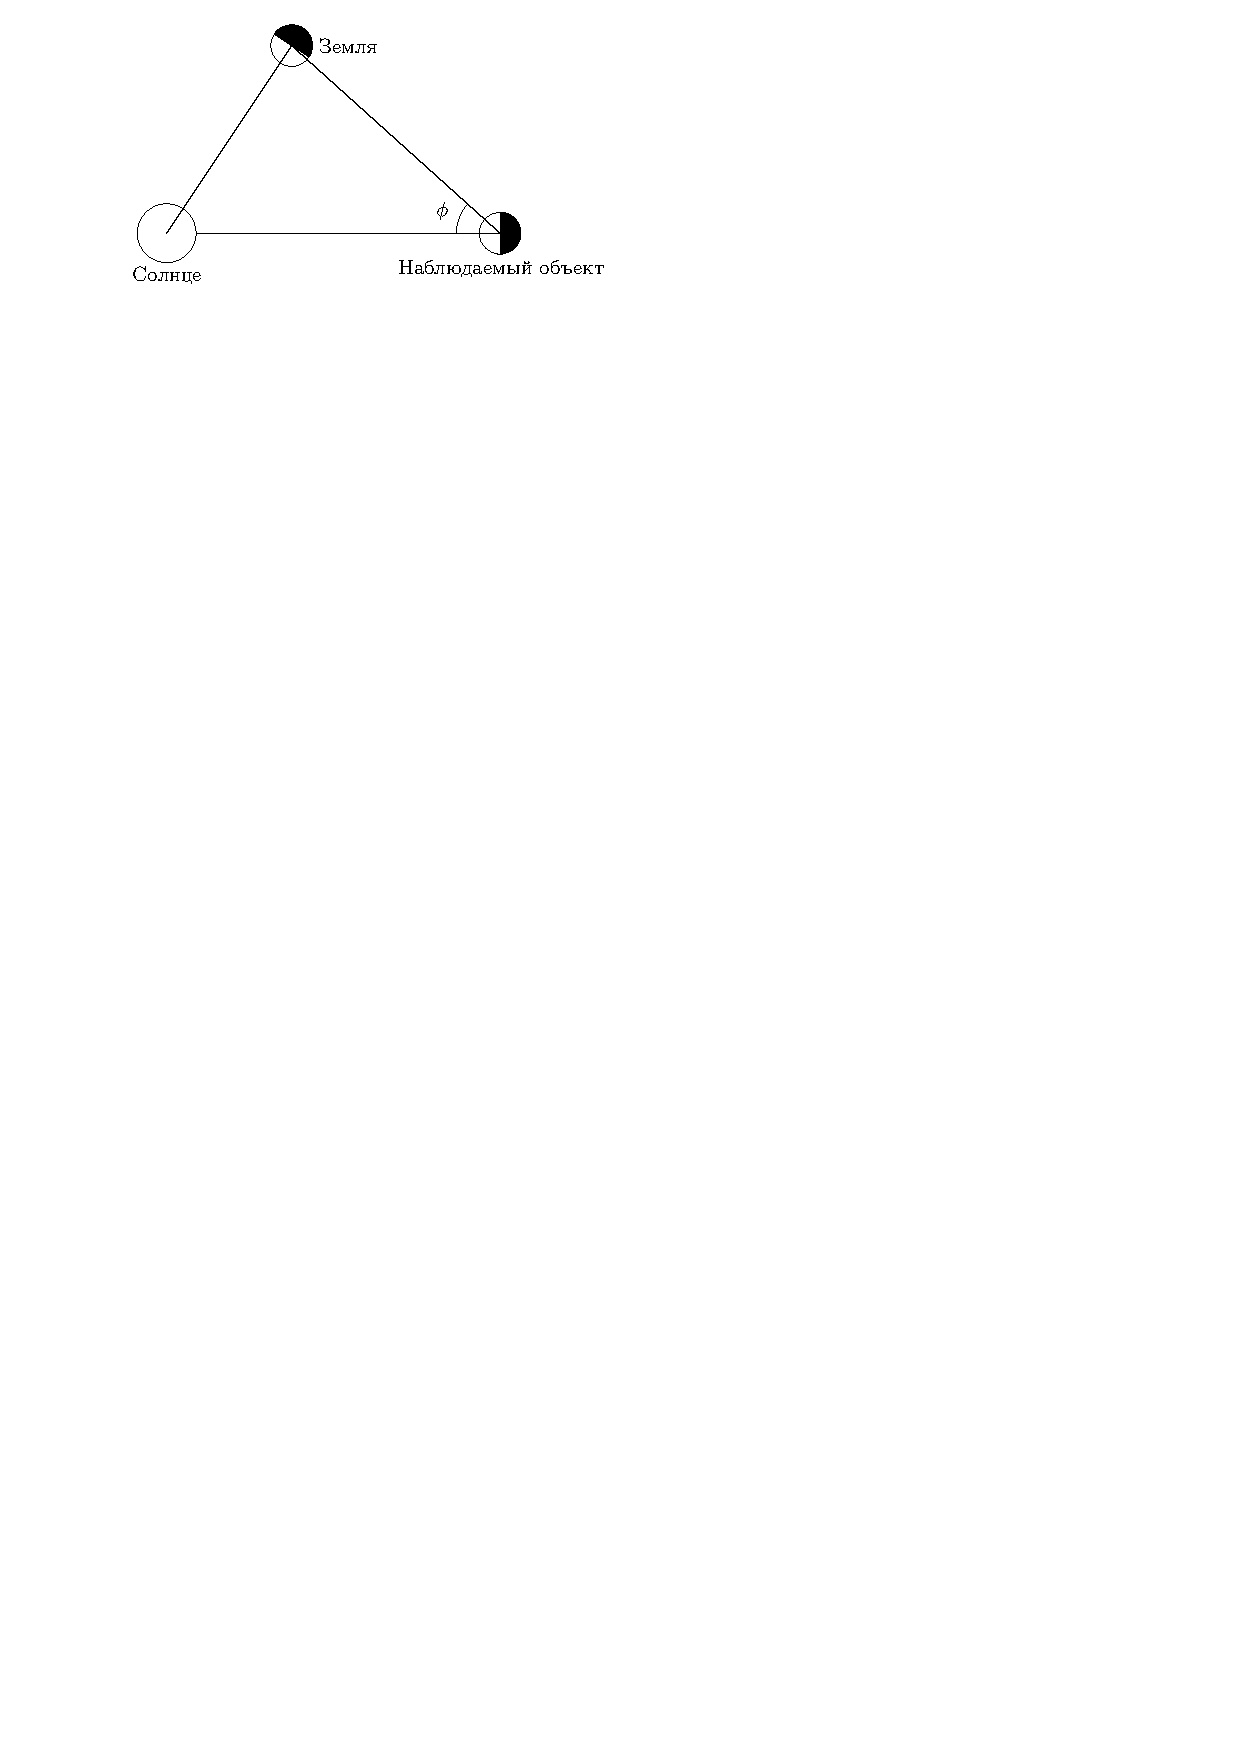
\includegraphics[width = 0.6\textwidth]{Phase_angle}
\begin{figure}[h!]
\caption{Фазовый угол}
\end{figure}
\end{center}